\documentclass[10pt]{extarticle}
\usepackage[a4paper,margin=1.6cm]{geometry}
\usepackage{amsmath,amssymb,bm,enumitem,titlesec,xcolor,booktabs,array,tikz}
\titleformat{\section}{\large\bfseries\color{blue!50!black}}{\thesection.}{0.5em}{}
\titlespacing*{\section}{0pt}{8pt}{3pt}
\setlist{nosep,leftmargin=1.3em}
\setlength{\parindent}{0pt}\setlength{\parskip}{4pt}
\newcommand{\B}{\mathbf B}\newcommand{\J}{\mathbf J}\newcommand{\Bo}{\mathbf B_{\rm obs}}
\pagestyle{plain}
\begin{document}
{\Large\bfseries A static magnetised solar atmosphere from a Bifrost snapshot}\\[2pt]
{\small What the M5h calculation does and why (physics explanation, B.Sc.\ level). HSEMHS code, 22 Oct 2026.}

\section{The question we are asking}
Bifrost is a computer simulation of the solar atmosphere: from below the visible surface up into the corona. One snapshot of it (run \texttt{en024048\_hion}, snapshot 385) gives us, at every point of a box, the temperature $T$, the gas pressure, the density and the magnetic field $\B$. In the simulation the gas is \emph{moving} (convection, waves, flows), so at any instant the forces on a parcel of gas do \textbf{not} cancel: the net force is what accelerates it.

We want a \textbf{static} (time-independent, no flows) atmosphere that looks as much as possible like this snapshot. ``Static'' means that at every point the forces on the gas add up to zero. We keep the Bifrost temperature exactly and keep the magnetic field \emph{close} to the Bifrost field, and we let the \emph{pressure} (and hence the density) adjust until the forces balance. Such a state is called \textbf{magnetohydrostatic (MHS)} equilibrium.

What we finally care about is the height of the visible ``surface'' of the Sun, the level $\tau_{500}=1$ (Sect.~7). Its height depends on the pressure. So we watch it during the calculation, and we say we are finished when it stops moving.

\section{The quantities}
\renewcommand{\arraystretch}{1.15}
\begin{tabular}{>{$}l<{$} p{9.6cm} l}
\toprule
\text{Symbol} & Meaning & Unit \\ \midrule
x,\,y & horizontal coordinates; the box is $24\times24$\,Mm, periodic (what leaves one side enters the other) & m \\
z & height; $z=0$ is roughly the solar surface, the box spans $-2.44$\,Mm to $+14.37$\,Mm & m \\
\hat{\mathbf z} & unit vector pointing up & -- \\
T & temperature, taken from Bifrost and \textbf{never changed}; 2400\,K to 1.6\,MK & K \\
P & gas pressure (the main unknown) & Pa = N\,m$^{-2}$ \\
\rho & mass density of the gas & kg\,m$^{-3}$ \\
g & solar surface gravity, $g=274$; gravity vector $\mathbf g=-g\,\hat{\mathbf z}$ & m\,s$^{-2}$ \\
\B & magnetic field (the second unknown); $10^{-4}$\,T $=1$\,G & T \\
\Bo & the Bifrost magnetic field (``observed'' field we want to stay close to) & T \\
\sigma & allowed deviation of $\B$ from $\Bo$: $\sigma=\sqrt{(0.05|\Bo|)^2+(5\,{\rm G})^2}$ & T \\
\mu_0 & vacuum permeability, $4\pi\times10^{-7}$ & T\,m\,A$^{-1}$ \\
\J & electric current density, $\J=\nabla\times\B/\mu_0$ (Amp\`ere's law) & A\,m$^{-2}$ \\
\mathbf A & magnetic vector potential, $\B=\nabla\times\mathbf A$ & T\,m \\
k_B,\ m_{\rm H} & Boltzmann constant; mass of a hydrogen atom & J\,K$^{-1}$, kg \\
\bar\mu & mean molecular weight: average particle mass in units of $m_{\rm H}$ (depends on ionisation) & -- \\
\chi_{500} & absorption (opacity) coefficient of the gas for light of wavelength 500\,nm & m$^{-1}$ \\
\tau_{500} & optical depth at 500\,nm, measured downward from the top (Sect.~7) & -- \\
z_{\tau1} & height where $\tau_{500}=1$ in a given vertical column & m \\
P_{\rm ref} & fixed pressure at the bottom of the box, $5.22\times10^6$\,Pa & Pa \\
\bottomrule
\end{tabular}

\section{The forces and the equilibrium equation}
Consider a small volume of gas. Three forces per unit volume (N\,m$^{-3}$) act on it:
\begin{enumerate}
\item \textbf{Gravity:} $\rho\,\mathbf g=-\rho g\,\hat{\mathbf z}$. It pulls the gas down.
\item \textbf{Pressure force:} $-\nabla P$. Gas is pushed from high to low pressure. If pressure falls with height, this force points up.
\item \textbf{Lorentz force:} $\J\times\B$, the force of the magnetic field on the currents flowing in the ionised gas. Using $\J=\nabla\times\B/\mu_0$ it can be written as
\[
\J\times\B=-\nabla\!\left(\frac{B^2}{2\mu_0}\right)+\frac{(\B\cdot\nabla)\B}{\mu_0},
\]
i.e.\ a \emph{magnetic pressure} $B^2/2\mu_0$ (field lines push apart) plus a \emph{magnetic tension} (bent field lines want to straighten, like stretched rubber bands).
\end{enumerate}
\textbf{Equilibrium (MHS):} the sum must vanish at every point,
\[
\boxed{\;-\nabla P+\J\times\B+\rho\,\mathbf g=0,\qquad \nabla\cdot\B=0\;}
\]
The second equation (Gauss's law for magnetism: no magnetic monopoles) must hold for any real magnetic field.

\textbf{Special case, no magnetic field (hydrostatic equilibrium, ``HSE'').} Only the vertical component remains: $dP/dz=-\rho g$. With the ideal gas law (next section) $\rho=\bar\mu m_{\rm H}P/(k_BT)$ this gives
\[
\frac{dP}{dz}=-\frac{P}{H},\qquad H=\frac{k_BT}{\bar\mu m_{\rm H}g},\qquad P(z)=P(z_0)\exp\!\Big(-\!\int_{z_0}^{z}\frac{dz'}{H}\Big).
\]
$H$ is the \textbf{pressure scale height}: the height over which $P$ drops by a factor $e$. In the photosphere ($T\approx6000$\,K, $\bar\mu\approx1.3$) $H\approx140$\,km; in the 1\,MK corona it is $\sim$50\,Mm. Because of this exponential, the pressure in our box spans about 12 orders of magnitude. This is why the code works with $u=\ln P$ rather than $P$ itself.

\textbf{Which force wins?} The ratio of gas to magnetic pressure is the \textbf{plasma beta}, $\beta=2\mu_0P/B^2$. Deep down $\beta\gg1$: the gas dominates and the field is pushed around by it. Higher up $\beta\ll1$: the field dominates. There, force balance is only possible if the field is nearly \emph{force-free} ($\J\times\B\approx0$, currents flow along field lines).

\section{Equation of state: how $\rho$ (and $\chi_{500}$) follow from $T$ and $P$}
To know the gravity force we need $\rho$. For an ideal gas $P=nk_BT$ with $n$ the number of particles per m$^3$, so
\[
\rho=\frac{\bar\mu\,m_{\rm H}\,P}{k_B T}.
\]
The difficulty is $\bar\mu$: when hydrogen ionises (around 6000--10\,000\,K) each atom becomes two particles (proton + electron) and $\bar\mu$ roughly halves. Molecules form in the coolest gas. How much is ionised depends on both $T$ and $P$ (Saha equation). We therefore use a pre-computed \textbf{equation-of-state (EOS) table} (Wittmann's code, solar composition). Given $(T,P)$ it returns $\rho$ and also the opacity $\chi_{500}$. The new table covers $T=2172$\,K--1.78\,MK and $P=10^{-13}$--$10^{15}$\,Pa, which encloses every point of the full Bifrost box. (The old table stopped at 1.61\,MK; that was the cause of the failed columns.)

\section{Why we cannot simply keep the Bifrost field}
We know $T$, and we have four unknown functions ($P$, $B_x$, $B_y$, $B_z$). The equations are the three components of the force balance plus $\nabla\cdot\B=0$.
\begin{itemize}
\item If we froze $\B=\Bo$, the pressure alone would have to cancel the Lorentz force. A gradient $\nabla P$ cannot balance an arbitrary force: the curl of a gradient is always zero, so the curl of ($\J\times\B+\rho\mathbf g$) would have to vanish, and for a snapshot of a moving atmosphere it does not.
\item So we must let \emph{both} $P$ and $\B$ change. We want $\B$ to move only as much as needed, ideally by less than $\sigma$ (5\,\% or 5\,G).
\end{itemize}
This turns the problem into a \textbf{compromise}: make the force imbalance as small as possible while keeping $\B$ close to $\Bo$. Mathematically this is a least-squares problem (Sect.~8).

\section{How the three field components $B_x$, $B_y$, $B_z$ are used}
\textbf{(a) What we are given.} The input file contains $B_{x,{\rm obs}}$, $B_{y,{\rm obs}}$, $B_{z,{\rm obs}}$ (tesla, $z$ positive upward) from Bifrost. They are given at the same points as $T$, the cell centres. For each point and each component the allowed deviation is the same number,
\[
\sigma=\sqrt{(0.05\,|\Bo|)^2+(5\times10^{-4}\,{\rm T})^2},\qquad |\Bo|=\sqrt{B_{x,{\rm obs}}^2+B_{y,{\rm obs}}^2+B_{z,{\rm obs}}^2},
\]
so a strong-field point may deviate by 5\,\%, and a weak-field point by about 5\,G. This is a chosen tolerance, not a measured error.

\textbf{(b) Where the model field lives (staggered grid).}\par\noindent
\begin{minipage}[t]{0.56\linewidth}\vspace{0pt}
Each component of the model field is stored on the cell face that it points through:
\begin{itemize}
\item $B_x$ on the faces perpendicular to $x$ (the left/right faces);
\item $B_y$ on the faces perpendicular to $y$ (front/back);
\item $B_z$ on the faces perpendicular to $z$ (bottom/top).
\end{itemize}
$B_x$ on a face is the magnetic flux through that face divided by its area. The total flux out of a cell is the sum over its six faces. For $\B=\nabla\times\mathbf A$ this sum is exactly zero (Stokes' theorem around the edges, every edge counted twice with opposite sign). So no cell can contain a ``magnetic charge''. The pressure $P$ and the density $\rho$ are at the cell centre. The currents $\J$ are on the cell edges (they circulate around the faces). The sketch shows a vertical $x$--$z$ slice.
\end{minipage}\hfill
\begin{minipage}[t]{0.40\linewidth}\vspace{0pt}\centering
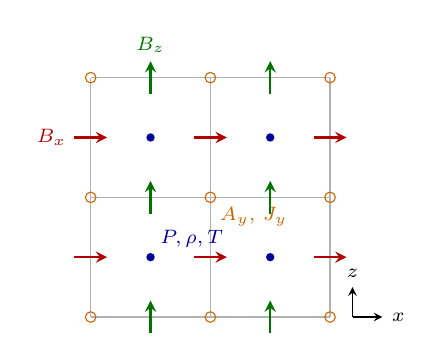
\begin{tikzpicture}[scale=0.95,>=stealth]
\draw[gray!60] (0,0) grid[step=1.6] (3.2,3.2);
\foreach \x in {0.8,2.4}\foreach \z in {0.8,2.4}{\fill[blue!60!black] (\x,\z) circle (1.6pt);}
\node[blue!60!black,font=\scriptsize,above right] at (0.8,0.8) {$P,\rho,T$};
\foreach \x in {0,1.6,3.2}\foreach \z in {0.8,2.4}{\draw[->,red!70!black,thick] (\x-0.22,\z)--(\x+0.22,\z);}
\node[red!70!black,font=\scriptsize,left] at (-0.2,2.4) {$B_x$};
\foreach \x in {0.8,2.4}\foreach \z in {0,1.6,3.2}{\draw[->,green!45!black,thick] (\x,\z-0.22)--(\x,\z+0.22);}
\node[green!45!black,font=\scriptsize,above] at (0.8,3.4) {$B_z$};
\foreach \x in {0,1.6,3.2}\foreach \z in {0,1.6,3.2}{\draw[orange!80!black] (\x,\z) circle (2pt);}
\node[orange!80!black,font=\scriptsize,below right] at (1.6,1.6) {$A_y,\,J_y$};
\draw[->] (3.5,0)--(3.9,0) node[right,font=\scriptsize]{$x$};
\draw[->] (3.5,0)--(3.5,0.4) node[above,font=\scriptsize]{$z$};
\end{tikzpicture}\\[-2pt]
{\scriptsize $B_y$, $A_x$, $A_z$, $J_x$, $J_z$ lie on the faces/edges not cut by this slice.}
\end{minipage}

\textbf{(c) How $B_x,B_y,B_z$ are built from the unknowns.} We never adjust $B_x,B_y,B_z$ directly. The unknown is the vector potential $\mathbf A=(A_x,A_y,A_z)$ on the edges, plus one number $\bar b$:
\[
B_x=\frac{\partial A_z}{\partial y}-\frac{\partial A_y}{\partial z},\qquad
B_y=\frac{\partial A_x}{\partial z}-\frac{\partial A_z}{\partial x},\qquad
B_z=\frac{\partial A_y}{\partial x}-\frac{\partial A_x}{\partial y}+\bar b .
\]
Each derivative is the difference of the two edge values bounding the face, divided by their distance. In a horizontally periodic box, $\partial A_y/\partial x-\partial A_x/\partial y$ averages to zero over any horizontal plane. So the curl alone cannot produce the net vertical flux through the box; $\bar b$ supplies it. It starts at the box-average of $B_{z,{\rm obs}}$ and is itself an unknown.

\textbf{(d) The currents.} From the face field we compute the current on each edge, $\J=\nabla\times\B/\mu_0$:
\[
J_x=\frac1{\mu_0}\Big(\frac{\partial B_z}{\partial y}-\frac{\partial B_y}{\partial z}\Big),\quad
J_y=\frac1{\mu_0}\Big(\frac{\partial B_x}{\partial z}-\frac{\partial B_z}{\partial x}\Big),\quad
J_z=\frac1{\mu_0}\Big(\frac{\partial B_y}{\partial x}-\frac{\partial B_x}{\partial y}\Big).
\]
Each is again a difference of neighbouring face values. So a current is a \emph{change} of the field across space: a uniform field carries no current, and a sheared or twisted field does.

\textbf{(e) How $B_x,B_y,B_z$ enter the force balance.} The three components of the force balance are checked on the three kinds of face: the $x$-equation on $x$-faces, $y$ on $y$-faces, and $z$ on the horizontal faces in the interior:
\[
\begin{aligned}
x:&\quad \frac{\partial P}{\partial x}-(J_yB_z-J_zB_y)=R_x,\\
y:&\quad \frac{\partial P}{\partial y}-(J_zB_x-J_xB_z)=R_y,\\
z:&\quad \frac{\partial P}{\partial z}+\rho g-(J_xB_y-J_yB_x)=R_z .
\end{aligned}
\]
On an $x$-face, $\partial P/\partial x$ is the difference of the two centre pressures on either side. $J_y,J_z$ are averaged from the two nearest edges. $B_y,B_z$ are not stored there, so they are averaged from the four nearest faces of their kind. Note that the force on the $x$-face involves only the \emph{other} two field components: a field along $x$ exerts no Lorentz force along $x$. $\rho$ on a $z$-face is the geometric mean of the two cells above and below.

\textbf{(f) How $B_x,B_y,B_z$ are compared with Bifrost.}
\begin{itemize}
\item \emph{Data term, on faces:} each face compares its own component with Bifrost interpolated to that face. For example, on the $x$-face between centres $i$ and $i{+}1$:
\[
c=\frac{B_x^{\rm face}-\tfrac12\big(B^{(i)}_{x,{\rm obs}}+B^{(i+1)}_{x,{\rm obs}}\big)}{\sqrt{\sigma^{(i)}\sigma^{(i+1)}}},\qquad \Phi_B=\langle c^2\rangle .
\]
$c$ counts how many $\sigma$ the model is off. All $x$-, $y$- and $z$-faces enter equally. At the top and bottom boundaries, $B_z$ is compared with the nearest centre value.
\item \emph{Smoothness term, at centres:} the model field is averaged back to the centres, e.g.\ $\tfrac12(B_x^{\rm left}+B_x^{\rm right})$. The difference $\delta\B=\B^{\rm centre}-\Bo$ is then required to vary smoothly: its second differences in $x$, $y$ and $z$, in units of $\sigma$, are penalised ($\Phi_S$). The model may differ from Bifrost by a smooth, large-scale correction, but not by cell-to-cell noise.
\item \emph{Grid-scale currents} ($\Phi_Q$): second differences of each current component along the grid are penalised. This prevents the field from balancing forces with unphysical zig-zag currents.
\end{itemize}

\textbf{(g) Where the field does \emph{not} enter.} The density, the opacity $\chi_{500}$ and hence $\tau_{500}$ and $z_{\tau1}$ depend only on $T$ and $P$. The field changes $z_{\tau1}$ only \emph{indirectly}: through the pressure the Lorentz force demands. Example: in a strong vertical flux tube (a magnetic element) the magnetic pressure $B^2/2\mu_0$ supports the tube against its surroundings, so the gas pressure inside must be lower. Less gas means lower opacity, so we see deeper there. In the Sun this is the Wilson depression.

\textbf{(h) First step for the field.} Before force balance is switched on, $\mathbf A$ is chosen so that the face fields match Bifrost as closely as possible (only $\Phi_B+\Phi_S$, pressure frozen). The match is excellent but not perfect: at the start only 0.004\,\% of faces are more than $3\sigma$ off, and the worst face is $15\sigma$ off.

\section{Optical depth and the height of the visible surface}
Light at 500\,nm travelling upward through the gas is absorbed. Over a small path $dz$ a fraction $\chi_{500}\,dz$ is lost. The \textbf{optical depth} counts, from the top of the atmosphere down to height $z$, how many ``absorption lengths'' the light must cross to escape:
\[
\tau_{500}(z)=\tau_{\rm top}+\int_{z}^{z_{\rm top}}\chi_{500}\big(T(z'),P(z')\big)\,dz'.
\]
Light emitted at depth $\tau$ escapes with probability $e^{-\tau}$. So what we see comes from around $\tau_{500}\approx1$. The height where $\tau_{500}=1$ ($\log_{10}\tau_{500}=0$) is the \textbf{visible surface}, $z_{\tau1}(x,y)$; it is a corrugated sheet, one height per vertical column. $\tau_{\rm top}$ is a small correction for the gas above the box: we assume $\chi$ keeps falling exponentially above the top, which gives $\tau_{\rm top}=\chi_{\rm top}H_\chi$ with $H_\chi$ the opacity scale height.

\textbf{Why $z_{\tau1}$ depends on the pressure.} $\chi_{500}$ grows steeply with density and with the number of free electrons (the main 500\,nm absorber in the photosphere is the H$^-$ ion, which needs free electrons). If the solution puts more gas in a column, $\tau=1$ is reached higher up; with less gas it is reached deeper. So $z_{\tau1}$ is a sensitive \emph{physical} probe of the pressure we compute. In the starting state (each column in HSE separately) the median $z_{\tau1}$ is 65\,km, ranging from $-143$ to $+151$\,km.

\section{The quantity that is minimised}
\textbf{Grid.} The box is cut into $504\times504\times496$ cells: 47.6\,km wide horizontally, 19--97\,km tall (finer near the surface). The pressure lives at cell centres. The magnetic field is stored as the vector potential $\mathbf A$ on cell edges, and $\B=\nabla\times\mathbf A$ (plus a constant vertical field $\bar b$) is computed on the cell faces. Because the divergence of a curl is identically zero, $\nabla\cdot\B=0$ is then \textbf{automatically exact}. We never have to enforce it. About $5\times10^8$ numbers are unknown.

\textbf{Force residual.} On every cell face we compute the net force, i.e.\ the left side of the MHS equation (sign reversed),
\[
\mathbf R=\nabla P-\rho\,\mathbf g-\J\times\B \qquad(\mathbf R=0 \text{ means perfect balance}),
\]
and measure it in units of the local weight of the gas, $S\approx\rho g$ (from the starting state; with a floor so that it never becomes tiny). Thus $R/S=1$ means ``the unbalanced force is as large as gravity itself''.

\textbf{The ``cost'' $\Phi$}, a single number that is zero only for a perfect static state that exactly reproduces Bifrost:
\[
\Phi=\underbrace{\lambda_F\Big\langle\frac{R^2}{S^2}\Big\rangle}_{\Phi_F:\ \text{forces}}
+\underbrace{\Big\langle\frac{(\B-\Bo)^2}{\sigma^2}\Big\rangle}_{\Phi_B:\ \text{stay close to Bifrost}}
+\underbrace{\Phi_Q}_{\text{no zig-zag currents}}
+\underbrace{\Phi_S}_{\text{smooth changes of }\B}
\]
\begin{itemize}
\item $\langle\cdot\rangle$ is the average over all faces (volume-weighted).
\item $\Phi_B=1$ means $\B$ differs from $\Bo$ by $1\sigma$ on average.
\item $\Phi_Q$ penalises currents that flip sign from one cell to the next. Those are numerical artefacts at the grid scale, not physics.
\item $\Phi_S$ asks that the change $\B-\Bo$ be smooth in space.
\item The weights $\lambda_F=10^{-4}$, $\lambda_Q=10^{-3}$, $\lambda_S=10^{-3}$ set the relative importance of the terms.
\end{itemize}

\section{How the computer finds the minimum}
\begin{enumerate}
\item \textbf{Start, pressure:} every vertical column is put in hydrostatic equilibrium on its own (Sect.~3, field ignored), with the bottom pressure fixed at $P_{\rm ref}$.
\item \textbf{Start, field:} with the pressure frozen, find the $\mathbf A$ whose curl best matches $\Bo$. This is a large linear least-squares problem, solved with conjugate gradients.
\item \textbf{Improve both together, step by step} (Gauss--Newton with a trust region). At the current state, approximate $\Phi$ by a quadratic function of a small change ($\delta\ln P$, $\delta\mathbf A$), i.e.\ linearise the forces. Compute the change that minimises this approximation, but allow it to be no larger than a ``trust radius''. Then evaluate the true $\Phi$ for the changed state:
  \begin{itemize}
  \item if $\Phi$ dropped (by about as much as predicted), \textbf{accept} the step and enlarge the radius;
  \item if not, reject it and shrink the radius.
  \end{itemize}
  Safety limits: in one step $P$ may change at most by a factor $e^5\approx148$ at any point, and it may never drop below $e^{-3}$ of its starting value. The bottom pressure stays fixed.
\item The work is split over 24 processes on 4 computers (each owns a $84\times126$-column block of the box).
\end{enumerate}

\section{When are we done? What we measure each step}
After every accepted step $n$ we recompute, for each of the $504\times504=254\,016$ columns, the visible-surface height $z_{\tau1}^{(n)}$, using the \emph{new} pressure. Then we take the largest change over all columns,
\[
dz_{\max}^{(n)}=\max_{\text{columns}}\big|\,z_{\tau1}^{(n)}-z_{\tau1}^{(n-1)}\big| .
\]
\textbf{Stop} when $dz_{\max}<1$\,mm on 3 accepted steps in a row, and every column has a valid $\tau_{500}=1$ crossing. Then the surface no longer moves, so the pressure near the surface has settled.

We also follow:
\begin{itemize}
\item $\Phi$ and its parts. Is the force imbalance going down? Is $\B$ still within $\sigma$ of Bifrost?
\item The largest single change of $P$ and $\B$ in the step.
\item The ratio of the actual to the predicted decrease of $\Phi$ (near 1 means the linear approximation is good).
\end{itemize}

\textbf{Status (17:48, 8 accepted steps).}
\begin{itemize}
\item $\Phi$ fell from $1.37\times10^5$ to $1.37\times10^4$, almost entirely in the force term.
\item The fit to Bifrost ($\Phi_B\approx0.017$) is still well within $\sigma$ on average.
\item The surface still moves by tens of km per step: $dz_{\max}=50$\,km, and the median height swings between about 30 and 60\,km.
\item The pressure is still being reorganised, and we are far from the 1\,mm criterion.
\end{itemize}
\end{document}
